%! TeX program = lualatex
\documentclass[notes, 10pt, aspectratio=169]{beamer}
%\documentclass[10pt, aspectratio=169]{beamer}

\usepackage{booktabs}
\usepackage[style=verbose,backend=biber]{biblatex}
\addbibresource{../snacspaper.bib}

% notes
\usepackage{pgfpages}
\setbeamertemplate{note page}[plain]
\setbeameroption{show notes on second screen=right}
\graphicspath{{graphics/}}

\usetheme[style=fwn]{leidenuniv}
\useinnertheme{circles}
\useoutertheme[subsection=false]{miniframes}
\beamertemplatenavigationsymbolsempty

% uncomment next line to let framesubtitle have palette primary color
%\setbeamercolor{framesubtitle}{use={palette primary},fg=palette primary.bg}

% uncomment next line to remove navigation symbols from the pdf
%\setbeamertemplate{navigation symbols}{}

\title{node2vec: Scalable Feature Learning for Networks}
\subtitle{Authors: Aditya Grover and Jure Leskovec}
\author{Chenyu Shi and Shupei Li}
\institute[LIACS]{Leiden Institute of Advanced Computer Science}
\date{November 18, 2022}


\begin{document}

\begin{frame}[plain]
	\titlepage
\end{frame}
\note{Hello, everyone! We are group 43. The paper we are going to present today is node2vec: scalable feature learning for networks, written by Grover and Leskovec.}

\begin{frame}
	\tableofcontents
\end{frame}
\note{This is a brief content of our presentation. Firstly, we will introduce some background knowledge about graph embeddings, followed by a review of related work. Then, we will explain the node2vec algorithm in detail and present experimental results in the original paper. After that, we will introduce the idea of our course project. This presentation is concluded with the future work we plan to do in the project.}

\section{Introduction}
\begin{frame}
    \frametitle{Introduction to Graph Embeddings}
    \begin{itemize}
        \item Represent graph-structured data.
        \item Applications: \\
            Social network analysis, recommender systems, molecular structure modelling, etc.
        \item Challenge: Limitations of traditional methods.
        \item Development of techniques specially for graph representations.\vspace{0.2cm}
            \begin{center}
                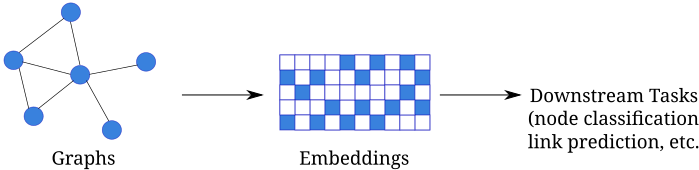
\includegraphics[width=10cm]{./graphics/intro.png}
            \end{center}
        \item node2vec is a feature learning framework.
    \end{itemize}
\end{frame}
\note{As we've seen in this course, complex relationships can be modelled by graphs. Graph-structured data appears in many modern applications like molecular structure modelling, social network analysis, recommender system, etc. However, if we want to leverage the information contained in graphs, we need to find a way to represent graph-structured data efficiently. Traditional statistical and machine learning methods are designed for extracting features from structured data, such as PCA, UMAP, t-SNE. Although these methods have achieved satisfactory performance on structured-data, they are hard to be generalized to graph-structured data, because they higly depend on properties of Eucildean space. This challenge led to the development of techniques specially for graph representation. Figure on the slide illustrates the general idea of graph embedding learning method. Firstly, we obtain embeddings by mapping graphs onto a low dimension space. And then, we can use these features in some downstream tasks like node classification and link prediction. From this perspective, node2vec algorithm that we address in presentation is a feature learning framework.}

\section{Related Work}
\begin{frame}
    \frametitle{Related Work}
    A taxonomy of graph embedding techniques \footcite{murphy2022}.
    \begin{center}
        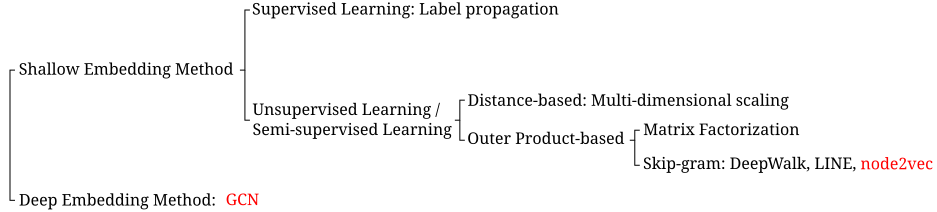
\includegraphics[width=14cm]{./graphics/related-work.png}
    \end{center}
\end{frame}
\note{This figure illustrates the taxonomy of graph embedding techniques, according to a textbook written by Murphy. There are two types of graph embedding techniques. They are shallow embedding method and deep embedding method. Shallow embedding methods use shallow encoding functions to map the original graph structure onto a Euclidean space and obtain the embedding matrix. If data is labelled, we can apply supervised algorithms to extract embeddings, for example, label propagation. However, labels are not avaliable or only partly avaliable in most cases, where we need to use unspervised or semi-supervised learning. These methods can be divided into distance-based method and outer product method further. Some representative algorithms are given in the figure. It is worth noting that node2vec algorithm we emphasize in presentation belongs to outer product-based method using skip-gram architecture, which is inspired by skip-gram model in natral language processing field. Deep embedding method usually refers to algorithms that learn graph features via graph neural networks, or GNN. GNN is a special class of artificial neural networks designed for graph-structured data. In our project experiments, we mainly use a method called graph convolutional networks, which is a popular GNN architecture.}

\section{Methodology}
\begin{frame}
    \frametitle{Feature Learning Framework}
    \begin{itemize}
    	\item node2vec is a feature learning framework in nature.
        \item Goal: Given a network $G=(V, E)$, find a projection $f:\ V \rightarrow R^d$.
        \item Generate a $d$-dimesion vector representation for each node.
        \item $f$ can be formulated as a matrix of size $\left| V \right| \cdot d$.
    \end{itemize}
\end{frame}
\note{Now we start to talk about methodology of node2vec. As we have shown on previous slides, node2vec is a feature learning framework in nature. So let’s give feature learning framework a formal defination. Feature learning framework aims to find a projection f,  which projects nodes set V to vector space. In other words, the task of a feature learning framework like node2vec is to generate a d-dimension embedding vector representation for each node. So, in mathematics form,  f can be formulated as a matrix of size v times d.
}

\begin{frame}
    \frametitle{Feature Learning Framework}
    \begin{columns}[t]
        \begin{column}{0.5\textwidth}
            Extending skip gram architecture to networks.\par ~\\
            Formulate feature learning in networks as a maximum likelihood optimization problem:
            \begin{align*}
                \max_{f}\ \sum_{u\in V}\log Pr\left( N_S\left( u \right)| f(u)  \right) 
            \end{align*}
            $N_S\left( a \right)$ is the network neighborhood set generated by neighborhood sampling strategy $S$ for node $a$.\par ~\\
            Important: $N_S\left( a \right)$ isn’t equavalent to direct local neighborhood.
        \end{column}
        \begin{column}{0.5\textwidth}
            For NLP: Given a literal data: \textit{This is a [feature learning \alert{framework} social network]}.
            \begin{align*}
                \scriptstyle
                Pr \left( \left\{ \text{"feature"}, \text{"learning"}, \text{"social"}, \text{"network"} \right\} | \text{"framework"} \right) 
            \end{align*}
            For Graph data: 
            \begin{align*}
                N_S\left( a \right) &= \left\{ b, c, d, e \right\} \\
            Pr\left( \left\{ b, c, d, e \right\}| a \right) &= Pr\left( N_s\left( a \right) | a \right) 
            \end{align*}
<<<<<<< HEAD
            Put that graph here!! 
            \note{So how to determine this projection f? Inspired by skip gram architecture in Natural language processing area, the authors formulate this problem as a maximum likelihood optimization problem. In NLP area, the given dataset contains literal data and we want to generate embedding vectors for each word. And skip gram architecture is to use a sliding window to obtain nearest neighbors for a word. Like here in the rightside example, in this sentence, feature - learning  - social - network is in the sliding window of the word framework. Then it computes and optimizes the likelihood probability for these four words in the sliding window to a maximum value. Then the literal structure information such as order of words in a sentence can be maintained most in the words embedding. In a similar way, now we are given a network data and wants to generate embedding vectors for each node. And at the same time we want our embedding to maintain as much as possible graph structure information. So we should have something similar to a sliding window in NLP problem. Perhaps for network data, it’s not as intuitional as NLP problem to define this sliding window.  In fact, the equavalent sliding window for network data is called network neighborhood Ns. Here please pay attention to definition of Ns. This network neighborhood isn’t equivalent to direct local neighborhood. We know the commonly used direct local neighborhood is totally decided by the graph structure. But this  Ns is not only related to the graph structure, but also related to a sampling strategy. And then we can compute the likelihood probability just like what we do in NLP area.}   
            \pause
            Two problems to be solved:
=======
            \begin{center}
                \vspace{-0.2cm}
                \includegraphics<1>[width=3.5cm, height=3cm]{./graphics/NLPGA.png}
            \end{center}
        \only<2>{Two problems to be solved:}
>>>>>>> 26a1ae693eb5ee920d088f444dae812deb3926ab
            \begin{enumerate}
                \item<2> How to define $N_S\left( a \right) $?
                \item<2> How to compute $Pr\left( N_S\left( a \right) |a \right) $?
            \end{enumerate}
        \end{column}
    \end{columns}
\end{frame}
\note{So here comes two key problems. First is how to define this network neighborhood and its corresponding sampling strategy S? The second is given Ns, how can we compute this likelihood probability for each node.
}

\begin{frame}
    \frametitle{Maximum Likehood Optimization}
    Formulate feature learning in networks as a maximum likelihood optimization problem:
    \begin{align*}
        \max_{f} \sum_{u\in V} \log Pr\left( N_S\left( u \right)|f(u)  \right) 
    \end{align*}
    Two standard assumptions:
    \begin{enumerate}
        \item Conditional independence:
            \begin{align*}
                Pr\left( N_S\left( u \right)| f\left( u \right)  \right) = \prod_{n_i\in N_S\left( u \right) }Pr\left( n_i|f(u) \right) 
            \end{align*}
        \item Symmetry in feature space:
            \begin{align*}
                Pr\left( n_i|f\left( u \right)  \right) = \frac{\exp\left( f\left( n_i \right) \cdot f\left( u \right)  \right) }{\sum_{v\in V}\exp\left( f\left( v \right)\cdot f\left( u \right)   \right)} 
            \end{align*}
    \end{enumerate}
\end{frame}
\note{Let’s see the second question first. To compute this formula, the authors made two assumptions to simplify the calculation. The first is conditional independence, which means the likelihood probablity to observe a neighborhood node is independent from observing any other neighborhood node. So because of the property of independent event, the likelihood probability can be rewritten in the form of this multiplication way. The second is symmetry in feature space, which means a source node and neighborhood node have a symmetric effect over each other in feature space. And then the authors model the likelihood probability for each pair of nodes as a softmax function.
}

\begin{frame}
    \frametitle{Maximum Likehood Optimization}
    Finally, the optimization problem is converted into the form of:
    \begin{align*}
        \max_f \sum_{u\in V} \left[ -\log\left( \sum_{u\in V}\exp\left( f(u)\cdot f(v) \right)  \right) + \sum_{n_i\in N_S(u)} f(n_i)\cdot f(u) \right] 
    \end{align*}
    Use stochastic gradient decent to obtain projection $f$.
\end{frame}
\note{So, with these two assumptions, the original optimization problem can be converted into the rightside formula. And for this formula, we can apply stochastic gradient decent method to obtain the optimal projection f.
}

\begin{frame}
    \frametitle{Network Neighborhood Sampling Strategy}
    Use classic search strategies:\\
    Breadth-first Sampling (BFS) and Depth-first Sampling (DFS).
    \begin{center}
        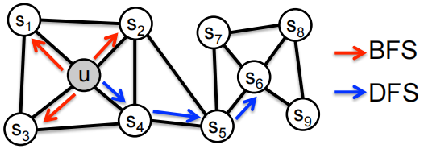
\includegraphics[width=6cm]{./graphics/BFS_DFS.png}
    \end{center}
    There are two kinds of similarities:
    \begin{enumerate}
        \item homophily (such as $u$ and $s_1$)
        \item structural equivalence (such as $u$ and $s_6$)
    \end{enumerate}
    \par \vspace{0.2cm}
    DFS tends to discover homophily, BFS tends to discover structural equivalence.\par \vspace{0.2cm}
    How to discover both kinds of similarities?
\end{frame}
\note{Now we come to the first problem, which is the most important part of node2vec, how to define sampling strategy and network neighborhood. Perhaps you are thinking why don’t we directly apply commonly used  local neighborhood as sliding window. That’s because there are two kinds of similarities, one is homophily, the other is structural equivalence. Let me explain in this example, homophily means two nodes are in the same group or community, such as u and s1. Structural equivalence means the nodes play a similar role in network, such as a bridge or a hub. The node u and s6 in this graph are both hub in their community so they share a structural equivalence. Directly applying local neighborhood is like using classic search strategy BFS, it tends to discover structural equivalence. On the contrary, there are another classic search strategy, DFS, tends to discover homophily. So, applying sampling method like this cannot discover both kind of two similarities at the same time and then fail to capture entire network features information. Therefore, we should come up with a better sampling method to combine BFS and DFS.
}


\begin{frame}
    \frametitle{Network Neighborhood Sampling Strategy}
    Use basic random walk to discover both homophily and structural equalvalence similarities.\par \vspace{0.2cm}
    Basic random walk with length $l$ from source node $u$:
    \begin{align*}
        P\left( c_i=x|c_{i-1}=v \right) =
        \begin{cases}
            \frac{\pi_{vx}}{Z}\qquad & \text{if } \left( v, x \right) \in E\\
            0\qquad & \text{otherwise}
        \end{cases}
    \end{align*}
    \begin{itemize}
        \item[] $c_i$: the $i$-th node in the walk.
        \item[] $v$: current node.
        \item[] $\pi_{vx}$: unnormalized transition probability.
        \item[] $Z$: normalization constant.
    \end{itemize}
\end{frame}
\note{Then we have a method called random walk which allows us to achieve it. Random walk is a method to take L steps to visit several nodes.  And we use the nodes which are visited in a walk as the network neighborhood of the source node. The most important thing for random walk is to decide which node to go in the next step. The formula on the slides gives out the transition probability. And you can see in this formula, there’s a pi v x, the unnormalized transition probability, needed to be determined.
}

\begin{frame}
    \frametitle{Network Neighborhood Sampling Strategy}
    \begin{columns}
        \begin{column}{0.5\textwidth}<1->
            $\pi_{vx}$: Often set $\pi_{vx}=w_{vx}$ in weighted graphs.\\
            \phantom{$\pi_{vx}$: }In unweighted graph: $\pi_{vx}=1$.
            \begin{center}
                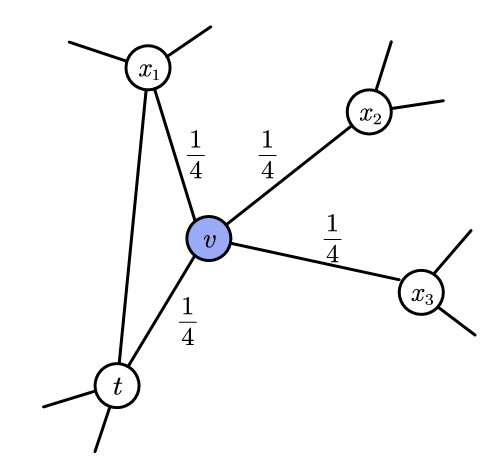
\includegraphics[width=5cm]{./graphics/Randomwalk.png}
            \end{center}
        \end{column}
        \note{Usually, the pi vx is set equal to the edge weight. And in unweighted garph, pi vx is set to 1, which means the all the neighborhood nodes will equally share the probability of being visited in the next step. So in this example, v is the current node, so node t and x1 2 3 will each have 1 over 4 probability to be visited in the next step.
        }
        \begin{column}{0.5\textwidth}<2->
            Random walk can combine features of DFS and BFS, and discovery both two kinds of similarities.\par ~\\
            Still not enough:\\
            It’s hard for us to guide and control the walking process.
        \end{column}
    \end{columns}
\end{frame}
\note{Random walk can allows us to visit and sample local nodes which are near to the source node, but also allows us to visit distant nodes which are far away from the source node. So it can combine features of DFS and BFS, and then can discover both kinds of similarities. But it’s still not enough. Because the entire walking process is random, it’s hard for us to guide and control the walking process.
}

\begin{frame}
    \frametitle{Network Neighborhood Sampling Strategy}
    \begin{columns}
        \begin{column}{0.5\textwidth}
         Use the second order bias random walk to get control of the walking process.
         \begin{align*}
             \pi_{vx} &= \alpha_{pq}\left( t, x \right) \cdot w_{vx}\\
             \alpha_{pq}\left( t, x \right) &=
             \begin{cases}
                 \frac{1}{p}\quad & \text{if } d_{tx} = 0\\
                 1\quad & \text{if } d_{tx} = 1\\
                 \frac{1}{q}\quad & \text{if } d_{tx} = 2
             \end{cases}
         \end{align*}
         \begin{itemize}
             \item[] $v$: current node.
             \item[] $t$: last node in the walk.
             \item[] $x$: next node to be chosen.
         \end{itemize}
        \end{column}
        \begin{column}{0.5\textwidth}
           \begin{center}
               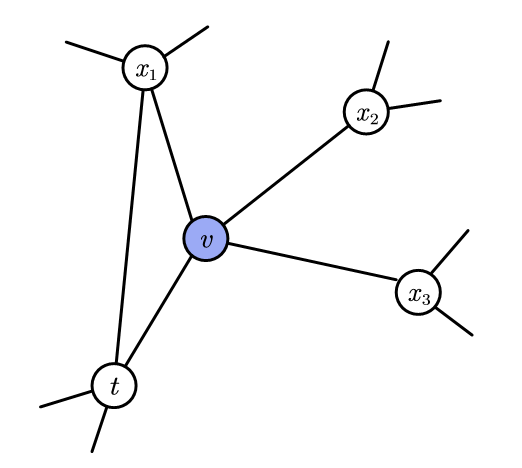
\includegraphics[width=5cm]{./graphics/graphexample.png}
           \end{center} 
        \end{column}
    \end{columns}
\end{frame}
\note{So the authors came up with an upgraded version, the second order bias random walk, which uses a bias value alpha, together with edge weight to decide the transition probability pi vx. And suppose currently we are in node v and want to decide which node to go in the next step. There are always three choices for us. The first choice is to step back, which means to return to node t, where we come from. The second is to stay around, which means to stay in the ego network of node t. The third choice is to go away, which means to go to a new node and jump out of the ego network of t. And in this second order bias random walk, we give these three choices different  transition probability. As you can see in the formula, dtx= zero one two means we choose to step back, stay around, and go away respectively. And these transition probability is controlled by two hyper parameters p and q}

\begin{frame}
    \frametitle{Network Neighborhood Sampling Strategy}
    \begin{columns}
        \begin{column}{0.5\textwidth}
            \begin{itemize}
                \item[] $p$: return parameter.
                \item[] $q$: in-out parameter.
            \end{itemize}
            \begin{center}
                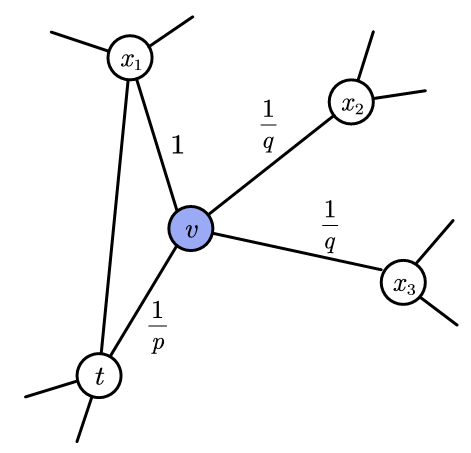
\includegraphics[width=5cm]{./graphics/biasrandomwalk.png}
            \end{center}
        \end{column}
        \begin{column}{0.5\textwidth}
            $p$ :
            \begin{itemize}
                \item High value: Less likely to sample
an already visited node.
                \item Low value: Likely to step back, then walk locally near the source node $u$.
            \end{itemize}
            $q$ :
            \begin{itemize}
                \item High value: Biased towards nodes close to $t$, act more similarly to BFS.
                \item Low value: Biased towards nodes distant to $t$, act more similarly to DFS.
            \end{itemize}
        \end{column}
    \end{columns}
\end{frame}
\note{And for this example graph, the unnormalized transition probability shall be like this. Through controlling the value of p and q, we can also get control of the walking process. For example, for p, a high value will decrease the transition probability to step back, then the sampling strategy is less likely to sample an already visited node. And for q, a high value will decrease the transition probability for the walk to go away. Then the walk process will be biased towards nodes close to t, and act more similarly to BFS. On the contrary, a low q value will make the walking process biased towards nodes distant from t, and act more similarly to DFS. 
}

\begin{frame}
    \frametitle{Learning Edge Features}
    We have found a projection $f: V\rightarrow R^d$ with node2vec, which allocates each node vector embedding representation.\par \vspace{0.2cm}
    These embedding vectors can be used in node-related downstream tasks.\par \vspace{0.2cm}
    But how to learn edge features and deal with edge-related downstream tasks?\pause
    \note{Up to now, we have worked out the two problems for node2vec. And then we can allocate each node a vector embedding representation, which can be used in node-related downstream task such as node classification. But how can we learn edge features and deal with edge-related downstream task?
    }
    \begin{center}
        \begin{tabular}{lll}
            \toprule
            \textbf{Operator} & \textbf{Symbol} & \textbf{Definition}\\
            \midrule
            Average & $\boxplus$ & $\left[ f(u)\boxplus f(v) \right]_i = \frac{f_i(u) + f_i(v)}{2}$\\
            Hadamard & $\boxdot$ & $\left[ f(u)\boxdot f(v) \right]_i = f_i(u) \ast f_i(v) $\\
            Weighted-L1 & $\left\Vert \cdot \right\Vert_{\bar{1}}$ & $\left\Vert f(u) \cdot f(v) \right\Vert_{\bar{1}_i} = \left| f_i(u) - f_i(v) \right|$  \\ 
            Weighted-L2 & $\left\Vert \cdot \right\Vert_{\bar{2}}$ & $\left\Vert f(u) \cdot f(v) \right\Vert_{\bar{2}_i} = \left| f_i(u) - f_i(v) \right|^2$\\
            \bottomrule
        \end{tabular}
    \end{center}
    Given projection $f$ obtained by node2vec and two nodes $u$, $v$ along with edge $(u,v)$, apply \\ the binary operator on $f(u)$ and $f(v)$ to generate the representation $g(u,v)$, where $g: V\times V\rightarrow R^{d^{'}}$.
\end{frame}
\note{The idea is very simple. Since each edge is composed of two nodes, so we can apply a binary operation to obtain a projection g and its corresponding edge embedding vectors. Here this table shows four commonly used binary operator. As long as we have obtained projection f, we can obtain projection g and edge embedding in this simple way. 
}

\section{Experiments}
\begin{frame}
    \frametitle{Experiment 1: Multi-label Classification}
    \begin{itemize}
        \item Task description
            \begin{itemize}
                \item[$\circ$] Labels from a finite set $\mathcal{L}$
                \item[$\circ$] Training: A fraction of nodes and all their labels.
                \item[$\circ$] Predict the labels for the remaining nodes.
            \end{itemize}
        \item Data\par
            ~\\
            \begin{tabular}{llll}
                \toprule
                \textbf{Dataset} & \textbf{Nodes} & \textbf{Edges} & \textbf{Labels}\\
                \midrule
                BlogCatalog & 10,312 & 333,983 & 39\\
                Protein-Protein Interactions (PPI) & 3,890 & 76,584 & 50\\
                Wikipedia & 4,777 & 184,812 & 40\\
                \bottomrule
            \end{tabular}
            \par~\\
        \item Metrics: Macro-F1 score.
    \end{itemize}
\end{frame}
\note{Authors of the original paper conducted two experiments to verify the effectiveness of the node2vec algorithm. The first experiment is multi-label classification. Given a finite label set and a fraction of nodes with labels, the task is predicting the labels for the remaining nodes. They use three data sets: BlogCatalog, PPI, and Wikipedia. The table shows some statistics of data sets. Macro-F1 score is selected as metrics.}

\begin{frame}
    \frametitle{Experiment 1: Multi-label Classification}
    \begin{itemize}
        \item Results\par
            ~\\
            \begin{tabular}{llll}
                \toprule
                \textbf{Algorithm} & & \textbf{Dataset} &\\
                             & BlogCatalog & PPI & Wikipedia\\
                \midrule
                Spectral Clustering & 0.0405 & 0.0681 & 0.0395\\
                DeepWalk & 0.2110 & 0.1768 & 0.1274\\
                LINE & 0.0784 & 0.1447 & 0.1164\\
                node2vec & \textbf{0.2581} & \textbf{0.1791} & \textbf{0.1552}\\
                \midrule
                node2vec settings (p, q) & 0.25, 0.25 & 4, 1 & 4, 0.5\\
                Gain of node2vec [\%] & \textbf{22.3} & \textbf{1.3} & \textbf{21.8}\\
                \bottomrule
            \end{tabular}
            \par~\\
        \item node2vec outperforms the other benchmark algorithms.
    \end{itemize}
\end{frame}
\note{Spectral clustering, DeepWalk, and LINE are selected as benchmarks. From the table, we can see that node2vec outperforms other algorithms on all datasets. Besides, its relative performance gain is significant.}

\begin{frame}
    \frametitle{Experiment 2: Link Prediction}
    \begin{itemize}
        \item Task description
            \begin{itemize}
                \item[$\circ$] A network with a fraction of edges removed.
                \item[$\circ$] Predict these missing edges.
            \end{itemize}
        \item Data\par
            ~\\
            \begin{tabular}{lll}
                \toprule
                \textbf{Dataset} & \textbf{Nodes} & \textbf{Edges}\\
                \midrule
                Facebook & 4,039 & 88,234 \\
                Protein-Protein Interactions (PPI) & 19,706 & 390,633\\
                arXiv ASTRO-PH & 18,722 & 198,110\\
                \bottomrule
            \end{tabular}
            \par~\\
        \item Metrics: Area Under Curve (AUC) score.
    \end{itemize}
\end{frame}
\note{The second task is link prediction. Given a network with a fraction of edges removed, the task is predicting these missing edges. They also use three datasets, Facebook, PPI, and arXiv, in this experiment. Statistics of data sets are shown in the table. AUC score is used as metrics.}

\begin{frame}
    \frametitle{Experiment 2: Link Prediction}
    \begin{itemize}
        \item Results\par
            ~\\
            \begin{tabular}{llll}
                \toprule
                \textbf{Algorithm} & & \textbf{Dataset} & \\
                             & Facebook & PPI & arXiv \\
                \midrule
                Common Neighbors & 0.8100 & 0.7142 & 0.8153\\
                Jaccard's Coefficient & 0.8880 & 0.7018 & 0.8067\\
                Adamic-Adar & 0.8289 & 0.7126 & 0.8315\\
                Pref. Attachment & 0.7137 & 0.6670 & 0.6996\\
                Spectral Clustering & 0.6192 & 0.4920 & 0.5740\\
                DeepWalk & \textbf{0.9680} & 0.7441 & 0.9340\\
                LINE & 0.9490 & 0.7249 & 0.8902\\
                node2vec & \textbf{0.9680} & \textbf{0.7719} & \textbf{0.9366}\\
                \bottomrule
            \end{tabular}
            \par~\\
        \item The learned feature representations outperform heuristic scores. node2vec achieves the best AUC.
    \end{itemize}
\end{frame}
\note{When the original paper was published, there were no feature learning algorithms that had been used for link prediction. Therefore, authors set four heuristic scores as benchmarks. The first four lines of table shows the performance of heuristic scores. The other three benchmarks are the same as in the experiment 1. Authors tested average, hadamard, weighted-L1, and weighted-L2 operations on these three benchmarks as well as node2vec. Due to the limited space, table on the slide only shows the result of hadamard operation. We can see that the learned feature representations outperform heuristic scores. And node2vec achieves the best AUC score on all datasets.}

\begin{frame}
    \frametitle{Summary of node2vec}
    \begin{itemize}
        \item An efficient graph embedding learning algorithm.
        \item Search strategy: Both flexible and controllable exploring network neighborhoods.
    \end{itemize}
\end{frame}
\note{A brief summary of node2vec. It is an algorithm designed for extracting embedidngs from graphs. Results of experiments support the effectiveness of the algorithm. Its neighborhood search strategy is flexible and controllable. We can easily change the behavior of search by adjusting hyperparameter p and q.}

\section{Our work}
\begin{frame}
    \frametitle{Our Contributions}
    \begin{enumerate}
        \item During the training of node2vec, the intermediate state of node embeddings is a black box.\par
        Our solution: Visualize the node embeddings during the training of node2vec with t-SNE technique.
        \item Randomly initialized inputs in GNN affect the robustness of model performance and extend the model training time.\par
            Our solution: Propose a novel method that combines node2vec and GNN.
        \item Effectiveness of algorithms.\par
            Our solution: Evaluate node2vec, GNN, and our proposed method on five real-world data sets with metrics that are different from the original paper.
    \end{enumerate}
\end{frame}
\note{Next, I will talk about our contributions in the project. Firstly, the intermediate state of node embeddings during node2vec training is a black box. We try to visualize the node embeddings with t-SNE technique to provide some insights into node2vec. Secondly, we find that researchers in graph embedding learning field have focused more on deep embedding methods these years. However, randomly initialized inputs in GNN affect the robustness of model performance and extend the training time. To address the problem, we proposed a novel method that combines node2vec and GNN. Thirdly, to further test the effectiveness of algorithms, we evaluate node2vec, GNN, and our proposed method on five real world datasets and select different metrics.}

\begin{frame}
   \begin{columns}
       \begin{column}{0.33\textwidth}
           \centering
           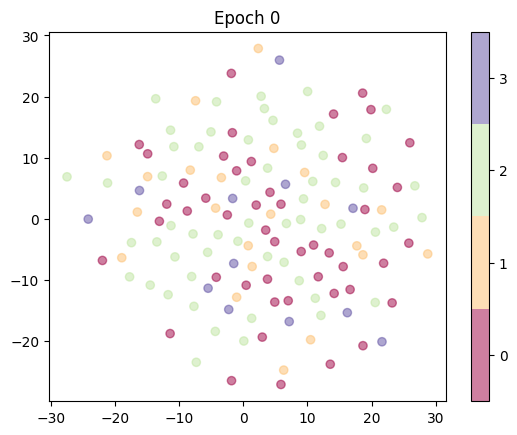
\includegraphics[width=0.9\textwidth]{./graphics/epoch0.png}
           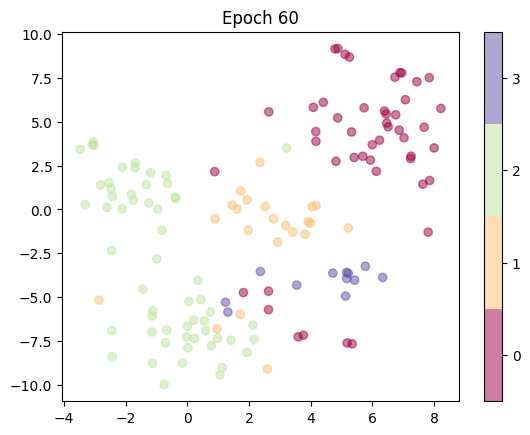
\includegraphics[width=0.9\textwidth]{./graphics/epoch60.png}
       \end{column}
       \begin{column}{0.33\textwidth}
           \centering
           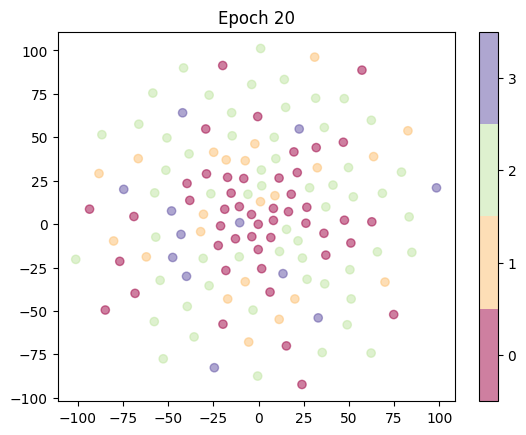
\includegraphics[width=0.9\textwidth]{./graphics/epoch20.png}
           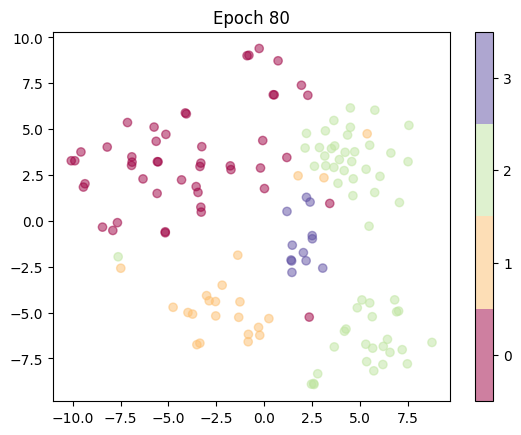
\includegraphics[width=0.9\textwidth]{./graphics/epoch80.png}
       \end{column}
       \begin{column}{0.33\textwidth}
           \centering
           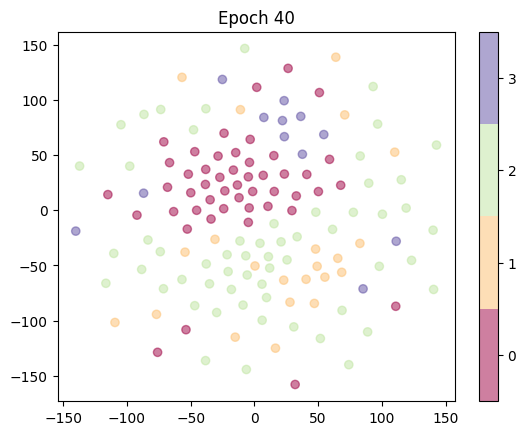
\includegraphics[width=0.9\textwidth]{./graphics/epoch40.png}
           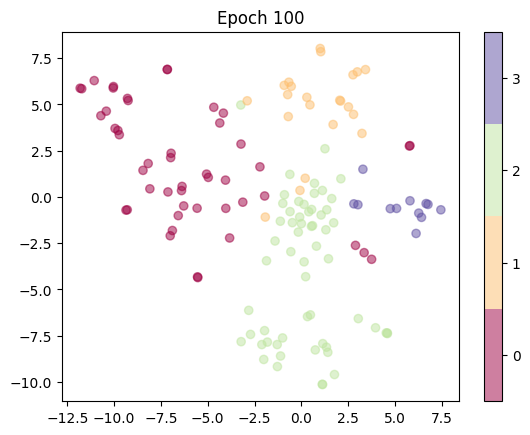
\includegraphics[width=0.9\textwidth]{./graphics/epoch100.png}
       \end{column}
   \end{columns} 
   \vspace{0.2cm}
   \begin{columns}
       \begin{column}{0.5\textwidth}
           AIFB dataset: Each node has a category label. There are 4 classes in total.
       \end{column}
       \begin{column}{0.5\textwidth}
           During the training of node2vec, nodes embedding are changed from chaos into order.
       \end{column}
   \end{columns}
\end{frame}
\note{We apply node2vec algorithm on an open source dataset AIFB. Results of visualization are showed on the slide. Each node in AIFB belongs to a class. The total number of classes is four. And we set the number of epochs to 100. It is easy to see that node embeddings are changed from chaos into order during the training of node2vec.}

\begin{frame}
    \frametitle{Proposed Method}
    \begin{columns}
        \begin{column}{0.7\textwidth}
            node2vec + GNN
            \begin{itemize}
                \item Inspired by the concept of meta learning.
                \item An improved version of GNN.
                \item Choose the graph convolutional network (GCN) in our experiments.
                    \begin{itemize}
                        \item[$\circ$] GCN iteration formula:
                            \begin{align*}
                                h^{(k)} = \sigma (\hat{D}^{-\frac{1}{2}}\hat{A}\hat{D}^{-\frac{1}{2}}h^{(k-1)}W^{(k)})
                            \end{align*}
                            with $\hat{A} = A + I$, where $A$ is the adjacency matrix and $\hat{D}$ is the diagonal node degree matrix of $\hat{A}$.
            \end{itemize}
    \end{itemize}
        \end{column}
        \begin{column}{0.3\textwidth}
           \begin{center}
               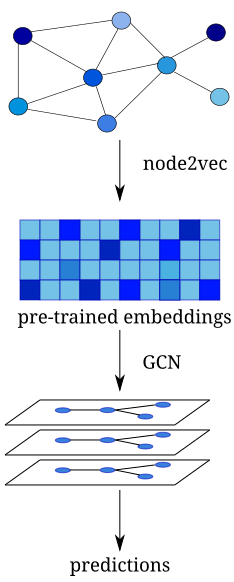
\includegraphics[height=6.5cm]{./graphics/proposed-model.png}
           \end{center} 
        \end{column}
    \end{columns}
\end{frame}
\note{As mentioned before, random initialization in GNN may not be a good strategy. Inspired by the concept of meta learning, we use the pretrained embeddings from node2vec as the meta information for GNN. Figure on the right illustrates the architecture of our proposed model. We expect our method will accelerate the training stage of GNN and improve the model performance. We choose graph convolutional network or GCN in our experiments. The iteration formula of GCN is given on the slide. Preliminary results we have obtained so far support the effectiveness of our proposed method.}

\section{Future work}
\begin{frame}
    \frametitle{Future work} 
    \begin{enumerate}
        \item Apply node2vec, GCN, and our proposed model to node classification and link prediction.
        \item Try different strategies of hyperparameter tuning.
    \end{enumerate}
\end{frame}
\note{Our future work will mainly focus on two tasks. Task one, apply node2vec, GCN, and our proposed model to node classification and link prediction. Task two, try different strategies of hyperparameter tuning. Due to the time limit, we omit technical details of GNN. If you are interested in GNN, we can discuss the principle of GNN together. Thank you. This's all of our presentation. Any questions?}

\section{Appendix}
\begin{frame}
    \frametitle{Graph Neural Network}
    \begin{columns}
        \begin{column}{0.5\textwidth}
            Graph Neural Network is a deep learning framework for graph.\par ~\\
            General GNN iteration formula:
            \begin{align*}
                \displaystyle
                h_u^{(k)} = \sigma (W_{\text{self}}^{(k)} h_u^{(k-1)} + W_n^{(k)}\sum_{v\in N(u)} h_v^{(k-1)} + b^{(k)} ) 
            \end{align*}
            \begin{itemize}
                \item[] $h_u^{(k)}$: $k$-th layer output embedding of node $u$.
                \item[] $W^{(k)}$: weights of $k$-th layer (trainable).
                \item[] $b^{(k)}$: bias of $k$-th layer (trainable).
                \item[] $\sigma$: activation function.
            \end{itemize}
        \end{column}
        \begin{column}{0.5\textwidth}
            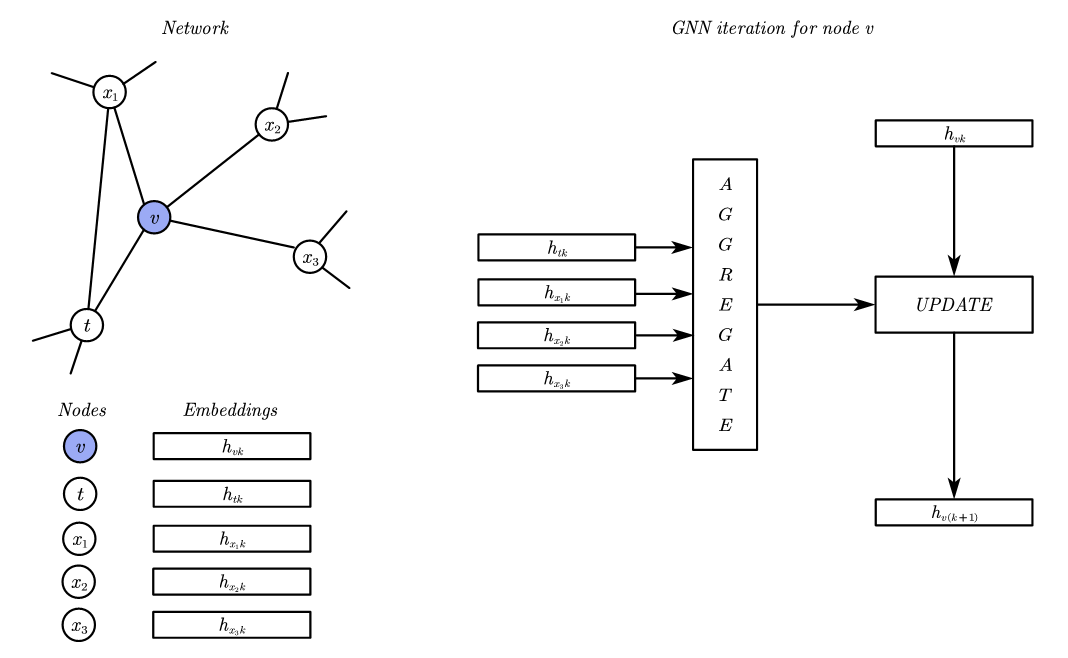
\includegraphics[width=7cm]{./graphics/gnn.png}
            Aggregate: To aggregate embeddings of $u$’s neighborhood.\par \vspace{0.2cm}
            Update: To update $u$’s embeddings using aggregation result and previous $u$’s embeddings.
        \end{column}
    \end{columns}
\end{frame}

\begin{frame}
    \frametitle{Graph Neural Network}
    \begin{align*}
        \displaystyle
        h_u^{(k)} = \sigma( W_{\text{self}}^{(k)} h_u^{(k-1)} + W_n^{(k)}\sum_{v\in N(u)} h_v^{(k-1)} + b^{(k)} ) 
    \end{align*}
    Final output embeddings can be used for calculating predictions. Then, we can use these predictions to compute the loss and optimize parameters with back propagation.\par \vspace{0.2cm}
    Problem: How to produce $h_u^0$ for each node?
    \begin{enumerate}
        \item Use one-hot vector for each node.
            \begin{itemize}
                \item[-] Drawback: The total number of nodes is large. Using one-hot vector for each node will cause the input tensor to be very sparse.
            \end{itemize} 
        \item Transfer pretrained embeddings from other similar tasks.
            \begin{itemize}
                \item[-] Drawback: There can't always be a similar task with pretrained embeddings for every network.
            \end{itemize}
        \item Use a trainable embedding layer to allocate randomly initialized embeddings for each node.
            \begin{itemize}
                \item[-] Drawback: Randomly initialized embeddings could have negative impact on training process.
            \end{itemize}
    \end{enumerate}
\end{frame}

\begin{frame}
    \frametitle{Combine node2vec and GNN}
    node2vec can produce embeddings for each node with graph information.\par ~\\
    GNN lacks a good general method to initialize its input nodes’ embeddings.\par ~\\
    We can use node2vec to produce initial input nodes’ embeddings for GNN to improve training process of GNN and obtain better performance.\par ~\\
    It’s a general method because there is no specific requirement of graphs when applying node2vec and GNN.
\end{frame}
\end{document}
